\section{Discussion: Rearrangements of Infinite Series}
    Consider the infinite series
    \begin{equation*}
        \sum_{n=1}^\infty\frac{(-1)^{n+1}}{n} = 1 - \frac{1}{2} + \frac{1}{3} - \frac{1}{4} + \frac{1}{5} - \frac{1}{6} + \dots 
    \end{equation*}
    If we just add from left to right, we get a series of \textit{partial sums}: $s_1 = 1,\; s_2 = 1/2,\; s_3 = 5/6$, and so on. We also see that the sums oscillate such that $s_1 > s_3 > s_5 > \dots$ and $s_2 < s_4 < s_6 < \dots$.
    \begin{center}
        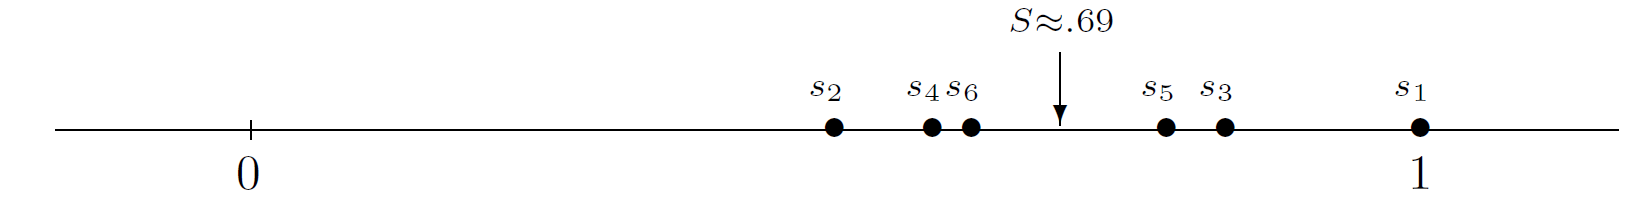
\includegraphics[width=200pt]{oscillating_converging.png}
    \end{center}
    
    